
\chapter{The Abstract Problem}\label{chap1}

SEVERAL\pageoriginale PROBLEMS IN the theory of Elasticity boil down
to the solution of a problem described, in an abstract manner, as
follows:

Let $V$ be a normed linear space over $\mathbb{R}$. Let $J:V\to
\mathbb{R}$ be a functional which can be written in the form
\begin{equation*}
J(v)=\frac{1}{2}a(v,v)-f(v)\quad \text{for all}\quad v\in
V,\tag{1.1}\label{chap1-eq1.1} 
\end{equation*}
where $a(\cdot,\cdot)$ is a continuous, symmetric bilinear form on $V$
and $f$ is an element of $V'$, the dual of $V$. Then the problem
consists in finding an element $u\in V$ such that
\begin{equation*}
J(u)=\Min_{v\in
    V}J(v).\tag{1.2}\label{chap1-eq1.2} 
\end{equation*}

Usually $J$ represents the {\em energy} of some physical system. 

More often, instead of minimising $J$ over the entire space $V$, we do
so over a non-empty convex subset $K$ of $V$ and find a element $u\in
K$ such that
\begin{equation*}
J(u)=\Min_{v\in K}J(v).\tag{1.3}\label{chap1-eq1.3}
\end{equation*}

Henceforth we shall denote this abstract problem by the symbol
$(P)$. One can ask immediately whether this problem admits of a
solution and if so, is the solution unique? We present in this section
the essential results regarding existence and uniqueness.

\begin{definition}\label{chap1-def1.1}
Let $V$ be a normed linear space. A bilinear form $a(\cdot,\cdot)$ on
$V$ is said to be $V$-elliptic if there exists a constant $\alpha>0$
such that for all $v\in V$.
\begin{equation*}
a(v,v)\geq \alpha || v ||^{2}.\tag{1.4}\label{chap1-eq1.4}
\end{equation*}\pageoriginale
\end{definition}

\begin{theorem}\label{chap1-thm1.1}
Let $V$ be a Banach space and $K$ a closed convex subset of $V$. Let
$a(\cdot,\cdot)$ be $V$-elliptic. Then there exists a unique solution
for the problem $(P)$.

Further this solution is characterised by the property:
\begin{equation*}
a(u,v-u)\geq f(v-u)\quad\text{for all}\quad v\in
K.\tag{1.5}\label{chap1-eq1.5} 
\end{equation*}
\end{theorem}

\begin{remark}\label{chap1-rem1.1}
The inequalities \eqref{chap1-eq1.5} are known as {\em variational
  inequalities}. 
\end{remark}

\begin{proof}
The $V$-ellipticity of $a(\cdot,\cdot)$ clearly implies that if
$a(v,v)=0$ then $v=0$. This together with the symmetry and bilinearity
of $a(\cdot,\cdot)$ shows that $a(\cdot,\cdot)$ defines an
inner-product on $V$. Further the continuity and the $V$-ellipticity
of $a(\cdot,\cdot)$ shows that the norm
\begin{equation*}
v\in V\to a(v,v)^{\frac{1}{2}}\tag{1.6}\label{chap1-eq1.6}
\end{equation*}
defined by the inner-product is equivalent to the existing norm on
$V$. Thus $V$ acquires the structure of a Hilbert space and we apply
the Riesz representation theorem to obtain the following: for all
$f\in V'$, there exists $\sigma f\in V$ such that
\begin{equation*}
f(v)=a(\sigma f,v)\quad\text{for all}\quad v\in
V.\tag{1.7}\label{chap1-eq1.7} 
\end{equation*}

The map $\sigma:V'\to V$ given by $f\mapsto \sigma f$ is linear. Now,
\begin{align*}
J(v) &=\frac{1}{2}a(v,v)-f(v)\\
     &= \frac{1}{2}a(v,v)-a(\sigma f,v)\\
     &= \frac{1}{2}a(v-\sigma f, v-\sigma f)-\frac{1}{2}a(\sigma
f,\sigma f).
\end{align*}

The symmetry of $a(\cdot,\cdot)$ is essential in obtaining the last
equality. For a given $f$,\pageoriginale since $\sigma f$ is fixed,
$J$ is minimised if and only if $a(v-\sigma f,v-\sigma f)$ is
minimised. But this being the distance between $v$ and $\sigma f$, our
knowledge of Hilbert space theory tells us that since $K$ is a closed
convex subset, there exists a unique element $u\in K$ such that this
minimum is obtained. This proves the existence and uniqueness of the
solution, which is merely the projection of $\sigma f$ over $K$.

We know that this projection is characterised by the inequalities:
\begin{equation*}
a(\sigma f-u,v-u)\leq 0\quad \text{for all}\quad v\in
K.\tag{1.8}\label{chap1-eq1.8} 
\end{equation*}

Geometrically, this means that the angle between the vectors $(\sigma
f-u)$ and $(v-u)$ is obtuse. See Fig.~\ref{chap1-fig1.1}.
\begin{figure}[H]
\centering
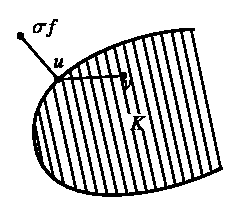
\includegraphics[scale=1.1]{figure/fig1.1.eps}
\caption{}\label{chap1-fig1.1}
\end{figure}

Thus, $a(\sigma f,v-u)\leq a(u,v-u)$ which by virtue of
\eqref{chap1-eq1.7} is precisely the relation
\eqref{chap1-eq1.5}. This completes the proof.
\end{proof}

We can state the following
\begin{corollary}\label{chap1-coro1.1}
\begin{enumerate}
\renewcommand{\theenumi}{\alph{enumi}}
\renewcommand{\labelenumi}{\rm(\theenumi)}
\item If $K$ is a non-empty closed convex cone with vertex at origin
  $0$, then the solution of $(P)$ is characterised by:
\begin{equation*}
\begin{cases}
a(u,v)\geq f(v)\quad\text{for all}\quad v\in K\\
a(u,u)=f(u).
\end{cases}\tag{1.9}\label{chap1-eq1.9}
\end{equation*}

\item If\pageoriginale $K$ is a subspace of $V$ then the solution is
  characterised by
\begin{equation*}
a(u,v)=f(v)\quad\text{for all}\quad v\in K.\tag{1.10}\label{chap1-eq1.10}
\end{equation*}
\end{enumerate}
\end{corollary}

\begin{remark}\label{chap1-rem1.2}
The relations \eqref{chap1-eq1.5}, \eqref{chap1-eq1.9} and
\eqref{chap1-eq1.10} are all called {\em variational formulations} of
the problem $(P)$.
\end{remark}

\begin{proof}
\begin{enumerate}
\renewcommand{\theenumi}{\alph{enumi}}
\renewcommand{\labelenumi}{(\theenumi)}
\item If $K$ is a cone with vertex at $0$, then for $u$, $v\in K$, $u+v\in
K$. (cf.\@ Fig.~\ref{chap1-fig1.2}). If $u$ is the solution to $(P)$, then for all
$v\in K$ applying \eqref{chap1-eq1.5} to $(u+v)$ we get $a(u,v)\geq
f(v)$ for all $v\in K$. In particular this applies to $u$
itself. Setting $v=0$ in \eqref{chap1-eq1.5} we get $-a(u,u)\geq
-f(u)$ which gives the reverse inequality necessary to complete the
proof of \eqref{chap1-eq1.9}. Conversely, if \eqref{chap1-eq1.9}
holds, we get \eqref{chap1-eq1.5} by just subtracting one inequality
from the other.
\begin{figure}[H]
\centering
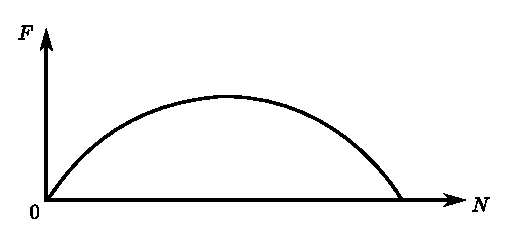
\includegraphics{figure/fig1.2.eps}
\caption{}\label{chap1-fig1.2}
\end{figure}

\item Applying (a) to $K$, since any subspace is a cone with vertex at
  $0$, we get (b) immediately. For if $v\in K$, then $-v\in K$ and
  applying \eqref{chap1-eq1.9} both to $v$ and $-v$ we get
  \eqref{chap1-eq1.10}. 
\end{enumerate}

This completes the proof.
\end{proof}

\begin{remark}\label{chap1-rem1.3}
The solution $u$ of $(P)$ corresponding to $f\in V'$ (for a fixed
$a(\cdot,\cdot)$) defines a map $V'\to V$. Since this solution is the
projection of $\sigma f$ on $K$, it follows that {\em the above map is
  linear if and only if $K$ is a subspace.} The problems associated
with variational inequalities are therefore nonlinear in general.
\end{remark}


\begin{exercise}\label{chap1-exer1.1}
Let\pageoriginale $V$ be as in Theorem \ref{chap1-thm1.1}. For
$f_{1}$, $f_{2}\in V'$, let $u_{1}$, $u_{2}$ be the corresponding
solutions of $(P)$. If $||\cdot ||^{\ast}$ denotes the norm in $V'$,
prove that
\begin{equation*}
||u_{1}-u_{2}||\leq \frac{1}{\alpha}||f_{1}-f_{2}||^{\ast}.
\end{equation*}
\end{exercise}

\begin{remark}\label{chap1-rem1.4}
The above exercise shows, in particular, the continuous dependence of
the solution of $f$, in the sense described above. This together with
the existence and uniqueness establishes that the problem $(P)$ is
``well-posed'' in the terminology of partial differential equations.
\end{remark}

\begin{exercise}\label{chap1-exer1.2}
If $V$ is a normed linear space, $K$ a given convex subset of $V$ and
$J:V\to \mathbb{R}$ any functional which is once differentiable
everywhere, then (i) if $u\in K$ is such that $J(u)=\Min\limits_{v\in
  K}J(v)$, $u$ satisfies, $J'(u)(v-u)\geq 0$ for all $v\in K$. (ii)
Conversely, if $u\in K$ such that $J'(u)(v-u)\geq 0$ for all $v\in K$,
and $J$ is everywhere twice differentiable with $J''$ satisfying
$J''(v)(w,w)\geq \alpha ||w||^{2}$, for all $v$, $w\in K$ and some
$\alpha\geq 0$, then $J(u)=\Min\limits_{v\in K}J(v)$.
\end{exercise}

\footnotetext[1]{Exercises \eqref{chap1-exer1.2}(i) and
  \ref{chap1-exer1.3} together   give relations \eqref{chap1-eq1.5}} 
\begin{exercise}[${}^1$]\label{chap1-exer1.3}
Apply the previous exercise to the functional
$$
J(v)=\frac{1}{2}a(v,v)=f(v)
$$
with $a(\cdot,\cdot)$ and $f$ as in Theorem \ref{chap1-thm1.1}. If $K$
is a subspace of $V$, show that $J'(u)(v)=0$ for all $v\in K$. In
particular if $K=V$, $J'(u)=0$.
\end{exercise}

It was essentially the symmetry of the bilinear form which provided
the Hilbert space structure in Theorem \ref{chap1-thm1.1}. We now drop
the symmetry assumption on $a(\cdot,\cdot)$ but we assume $V$ to be a
Hilbert space. In addition we assume that $K=V$.

\begin{theorem}[LAX-MILGRAM LEMMA]\label{chap1-thm1.2}
Let\pageoriginale $V$ be a Hilbert space. $a(\cdot,\cdot)$ a
continuous, bilinear, $V$-elliptic form, $f\in V'$. If $(P)$ is the
problem: to find $u\in V$ such that for all $v\in V$,
\begin{equation*}
a(u,v)=f(v),\tag{1.11}\label{chap1-eq1.11}
\end{equation*}
then $(P)$ has a unique solution in $V$\footnote[1]{cf.\@ Corollary
  \ref{chap1-coro1.1}(b).}. 
\end{theorem}

\begin{proof}
Since $a(\cdot,\cdot)$ is continuous and $V$-elliptic, there are
constants $M$, $\alpha>0$ such that
\begin{equation*}
\begin{split}
& |a(u,v)|\leq M||u||~||v||,\\
& a(v,v)\geq\alpha||v||^{2},
\end{split}\tag{1.12}\label{chap1-eq1.12}
\end{equation*}
for all $u$, $v\in V$. Fix any $u\in V$. Then the map $v\mapsto
a(u,v)$ is continuous and linear. Let us denote it by $\Au\in V'$. Thus
we have a map $A:V\to V'$ defined by $u\mapsto \Au$.
\begin{equation*}
||\Au||^{\ast} =\sup_{\substack{v\in V\\ v\neq
    0}}\frac{|\Au(v)|}{||v||}=\sup_{\substack{v\in V\\ v\neq
    0}}\frac{|a(u,v)|}{||v||}\leq
M||u||.\tag{1.13}\label{chap1-eq1.13} 
\end{equation*}

Thus $A$ is continuous and $||A||\leq M$.

We are required to solve the equation
\begin{equation*}
\Au=f.\tag{1.14}\label{chap1-eq1.14}
\end{equation*}

Let $\tau$ be the Riesz isometry, $\tau:V'\to V$ so that
\begin{equation*}
f(v)=((\tau f,v)),\tag{1.15}\label{chap1-eq1.15}
\end{equation*}
where $((\cdot,\cdot))$ denotes the inner product in $V$. Then,
$\Au=f$ if and only if $\tau \Au=\tau f$ or equivalently.
\begin{equation*}
u=u-\rho(\tau \Au-\tau f),\tag{1.16}\label{chap1-eq1.16}
\end{equation*}\pageoriginale
where $\rho>0$ is a constant to be specified. We choose $\rho$ such
that $g:V\to V$ is a contraction map, where $g$ is defined by
\begin{equation*}
g(v)=v-\rho(\tau Av-\tau f)\quad\text{for}\quad v\in
V.\tag{1.17}\label{chap1-eq1.17} 
\end{equation*}

Then the solution to $(P)$ will be the unique fixed point of this
contraction map, which exists by the contraction mapping theorem.

Let $v_{1}$, $v_{2}\in V$. Set $v=v_{1}-v_{2}$. Then
\begin{align*}
||g(v_{1})-g(v_{2})|| &= ||(v_{1}-v_{2})-\rho\tau A(v_{1}-v_{2})||\\
&= ||v-\rho \tau Av||.
\end{align*}

But,
\begin{align*}
||v-\rho \tau Av||^{2} &= ((v-\rho \tau Av, v-\rho \tau Av))\\
&= ||v||^{2}-2\rho((\tau Av,v))+\rho^{2}||\tau Av||^{2}\\
&= ||v||^{2}-2\rho Av(v)+\rho^{2}||Av||^{\ast^2}\\
&\leq ||v||^{2}-2\rho\alpha||v||^{2}+\rho^{2}M^{2}||v||^{2}\\
&= (1-2\rho\alpha+\rho^{2}M^{2})||v||^{2}
\end{align*}
since $Av(v)=a(v,v)\geq \alpha||v||^{2}$ and $||A||\leq M$. Choosing
$\rho\in ]0$, $\dfrac{2\alpha}{M^{2}}[$, we get that
\begin{equation*}
1-2\rho\alpha+\rho^{2}M^{2}<1\tag{1.18}\label{chap1-eq1.18}
\end{equation*}
and hence $g$ is a contraction, thus completing the proof.
\end{proof}

\begin{remark}\label{chap1-rem1.5}
The problem $(P)$ of Theorem \ref{chap1-thm1.2} is well-posed. The
existence and uniqueness were proved in the theorem. For the
continuous dependence of $u$ on $f$, we have
\begin{equation*}
\alpha||u||^{2}\leq a(u,u)=f(u)\leq ||f||^{\ast}\cdot
||u||.\tag{1.19}\label{chap1-eq1.19} 
\end{equation*}\pageoriginale
\end{remark}

\medskip
\noindent
{\bf REFERENCE.}~ For Variational Inequalities, see Lions and
Stampacchia \cite{key18}. 

